\hypertarget{Introduction}{%
\chapter{Introduction}\label{Introduction}}

\section{Présentation de la structure
d'accueil}

Durant la période de mon stage , j'ai été accueilli au
\textbf{Laboratoire de Mathématiques Informatique et Application
(LAMIA)} de l'Université des Antilles (UA).

Pour présenter cette structure, il me faut tout d'abord présenter
l'Université à laquelle il est rattaché.

\hypertarget{lUniversite-des-antilles}{%
\subsection{L'Université des Antilles}\label{luniversite-des-antilles}}

Voici quelques chiffres que je ne connaissais pas et qui donnent la
mesure de sa taille :

L'Université des Antilles s'organise autour deux pôles universitaires
régionaux autonomes : le « Pôle Guadeloupe » et le « Pôle Martinique ».

Sur ces pôles, l'Université assure des missions d'\emph{enseignement} et
de \emph{recherche}, assistées par des \emph{administratifs et des
techniciens}.

\hypertarget{administration-et-personnel-technique}{%
\subsubsection{Administration et personnel
technique}
\label{administration-et-personnel-technique}}

l'UA emploie 414 Administratifs et Techniciens (environ 200 personnes
pour l'administation centrale et 100 répartis sur chaque pôle)

\hypertarget{enseignements}{%
\subsubsection{Enseignements}\label{enseignements}}

L'UA délivre des diplomes de la licence au doctorat dans de nombreux
domaines. Au total, cela représente :

\begin{itemize}
\tightlist
\item
  484 enseignants-chercheurs (environ 240 pour chaque pôle)
\item
  12 000 étudiants (environ 7000 pour la Guadeloupe , 5000 pour la
  Martinique)
\end{itemize}

Pour l'informatique, cela représente : - autour de 20
enseignants-chercheurs - autour de 120 étudiants

\hypertarget{recherche}{%
\subsubsection{Recherche}\label{recherche}}

La recherche est structurée en laboratoires auxquels sont rattachés les
enseignants chercheurs qui peuvent former de futurs chercheurs : les
doctorants.

L'Université compte ainsi au total :

\begin{itemize}
\tightlist
\item
  17 laboratoires
\item
  320 doctorants
\end{itemize}

Pour ma part, comme signalé précédemment, j'ai effectué mon stage dans
le laboratoire LAMIA que je vais maintenant présenter.

\hypertarget{le-lamia}{%
\subsection{Le laboratoire LAMIA}\label{le-lamia}}

Le \textbf{Laboratoire de Mathématiques Informatique et Application
(LAMIA)}, comme son nom l'indique, se concentre sur les recherches en
informatiques et mathématiques.

Il compte une soixantaine de membres (Professeurs des Universités,
Maitres de Conférences, ATER, Doctorants) répartis sur deux pôles
(Guadeloupe et Martinique) au sein de trois équipes internes :

\begin{itemize}
\tightlist
\item
  Equipe
  \href{http://lamia.univ-ag.fr/index.php?page=equipe-mathematiques}{\textbf{Mathématiques}
  (analyse variationnelle, analyse numérique, EDP, analyse statistique,
  mathématiques discrètes)} ;
\item
  Equipe Informatique
  \href{http://lamia.univ-ag.fr/index.php?page=equipe-danais}{\textbf{DANAIS}
  : Data analytics and big data gathering with sensors} ;
\item
  Equipe Informatique
  \href{http://lamia.univ-ag.fr/index.php?page=equipe-aid}{\textbf{AID}
  : Apprentissages Interactions Donnees} ;
\end{itemize}

De plus, le LAMIA accueille en son sein un groupe de chercheurs associés
travaillant en Epidémiologie clinique et médecine.

L'équipe avec laquelle j'ai principalement travaillé est
celle d'\textbf{Apprentissages Interactions Données} qui développe des
méthodes de traitements et d'analyse de données hétérogènes : images
(classique, multi-spectrale), séquences vidéos, séries temporelles et
spatio-temporelles, dont la responsable est \textbf{Mme. Hélène
Paugam-Moisy}.

Indépendamment de ces équipes, les travaux de recherche du laboratoire
se répartissent en \textbf{projets} qui peuvent réunir des membres de
plusieurs équipes en \textbf{groupes de travail}. Mon stage était en
fait plus attaché à un projet et un groupe de travail qu'à une équipe.

Ce projet est nommé de façon informelle projet \textbf{``Spikes''} et
concerne l'utilisation de \textbf{réseaux de neurones impulsionnels}
pour l'apprentissage automatique (ces notions seront définies plus
loin). Le groupe de travail associé réunit à l'heure actuelle :

\begin{itemize}
\tightlist
\item
  1 Professeur des Universités
\item
  2 MCF avec HDR
\item
  3 MCF
\item
  1 ingénieur d'études.
\end{itemize}.

C'est avec ces personnes que j'ai travaillé tout au long du stage et mes
tuteurs de stage était \textbf{M.~Vincent PAGÉ et M. ~Manuel CLERGUE}.

Ci dessous, un schéma présentant la structure du laboratoire me
rattachement à cette structure. (L'équipe de travail \textbf{Spikestrain}
étant informelle, elle ne figure pas sur ce schéma.)

\begin{figure}[h!]
\centering
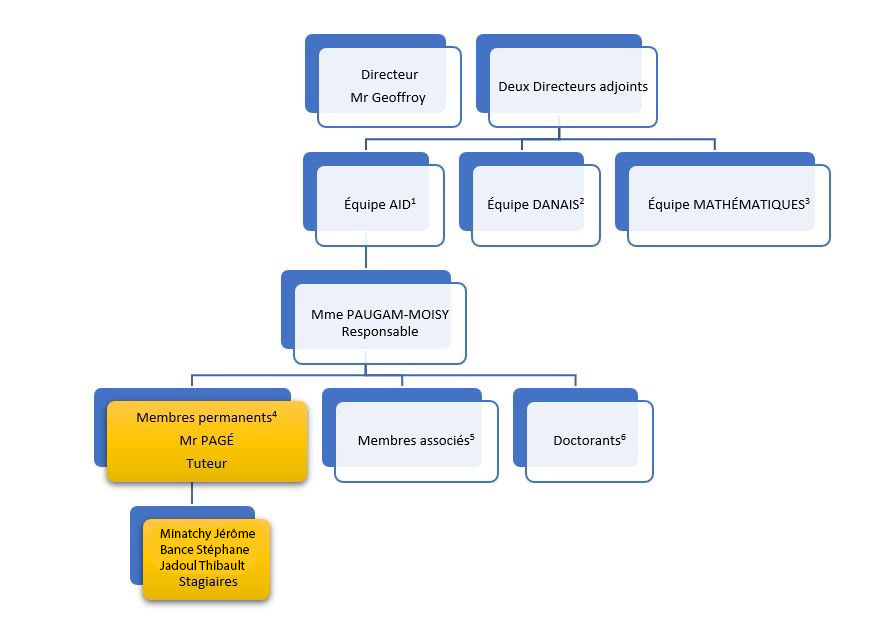
\includegraphics[width=10cm]{./images/orga.jpg}
\caption{Figure 1 Schéma de l'organisation interne du LAMIA:
¹Apprentissages Interactions Données. ²Data analytics and big data
gathering with sensors. ³Mathématiques (analyse variationnelle, analyse
numérique, EDP, analyse statistique, mathématiques discrètes). ⁴Membres
permanents : Suzy Gaucher-Casalis~(MCF),~Enguerran
Grandchamp~(MCF--HDR),~Jean-Luc Henry~(MCF),~Jimmy Nagau~(MCF),~Vincent
Pagé(MCF),~Helene Paugam Moisy~(PR),~Sébastien Régis~(MCF),~Céline
Rémi~(MCF).}
\end{figure}

La prochaine section sera consacrée à la présentation de la thématique
de recherche du groupe ``Spikestrain'' et de mon stage.


\hypertarget{Objectif_Spike}{%
\subsection{Le groupe Spiketrain}\label{Groupe_Spiketrain}}

Le groupe \textbf{Spikestrain} s'intéresse aux techniques
d'\textbf{Intelligence Artificielle}, plus spécifiquement à
l'\textbf{apprentissage automatique} dont l'objectif est de créer des
programmes capable d'apprendre à partir de bases d'exemples.

Actuellement, parmi les techniques permettant l'apprentissage
automatique , une se démarque et est très populaire : les
\textbf{réseaux de neurones artificiels} , notamment dans leur version
\emph{profonde} qui sont très utilisé par exemple par \textbf{Facebook™}
pour sa \textbf{reconnaissance faciale} ou encore par \textbf{Google™}
pour ses \textbf{robots} qui apprennent par \textbf{répétitions} à jouer
(échecs, Go).


\hypertarget{Contexte}{%
\section{Contexte du stage}\label{Contexte}}

\hypertarget{Le-Challenge}{%
\subsection{Le Challenge: Classifier les Cachalots}\label{Le-Challenge}}

Le challenge "Dyni Odontocete Click Classification, 10 species [ DOCC10 ]
by Universite de Toulon" (https://challengedata.ens.fr/challenges/32) consistait simplement à réaliser un classifieur qui classe des mammifères marins en une dizaine d'espèces à partir de leurs "Clics" pour celà nous avions à disposition une base d'apprentissage labelisée ainsi qu'une base de test non labelisée sur laquelle nous pouvions évaluer les performances réelles de nos classifieurs. Pour cela nous labelision les exemples de la base non labelisée puis nous envoyions nos prédictions sur le site du challenge qui nous renvoyais nos performances ainsi qu'un classement des performances de tous les participants.

Les deux bases sont consitituées d'enregistrements audios des clics des différentes espèces. Chaque enregistrement contient 8192 mesures faites à une fréquence d'échantillonnage de 200Hz. Dans le cas de la base non labelisée appellée base de test chaque enregistrement contient normalement un clic centré au milieu de la fenêtre tandis que dans la base labelisée appellée base d'apprentissage le clic n'est pas spécialement centré et peut se situer à divers moments de l'enregistrement de plus ceux ci peuvent contenir divers bruits.

L'objectif est de classer chaque enregistrement en fonction de l'espèce émettrice correspondante. Les 10 espèces sont : (0) Gg : Grampus griseus- Dauphin de Risso (1) Gma : Globicephala macrorhynchus- Baleine pilote à nageoires courtes (2) La : Lagenorhynchus acutus- Dauphin à flancs blancs de l'Atlantique (3) Mb : Mesoplodon bidens- Baleine à bec de Sowerby (4) Me : Mesoplodon europaeus- Baleine à bec de Gervais (5) Pm : Physeter macrocephalus - Cachalot (6) Ssp : Stenella sp.Dauphin stenellide (7) UDA : Delphinidés de type A - un groupe de dauphins (espèces non encore déterminées) (8) UDB : Delphinidés de type B - un autre groupe de dauphins (espèces non encore déterminées) (9) Zc : Ziphius cavirostris - Baleine de Cuvier à bec. La précision est de l'ordre du métre.


\hypertarget{Etat-des-lieux-lors-de-mon-arrivuxe9}{%
\subsection{Etat des lieux a mon arrivé}
\label{Etat-des-lieux-lors-de-mon-arrivuxe9}}

Quand j'ai commencé mon stage mes tuteurs avaient déjà commencé le challenge depuis un moment déjà c'est pourquoi j'ai dû dans un premier temps me mettre à jour sur le challenge et ce qu'ils avaient fait, à savoir :

-Un grand nombre de tentatives de résolution du probléme uniquement basé sur du machine learning notament des réseaux de neurones et des réseaux de neurones convolitifs
-De la Data Augmentation
-Divers traitements du signal

Leurs meilleurs résultats étaient de l'ordre de 95 pourcents de réussite sur la base labelisée contre 72 pourcents de réussite sur la base non labelisée, soit un écart de 20 pourcents de réussite entre les deux bases qui persistait même en utilisant d'autres méthodes de machine learning donnant de moins bons résultats.
Cet important différentiel est d'autant plus surprenant que les auteurs du challenge nous présentent les données de la base non labelisée comme des données de meilleures qualité que celles de la base labelisée.

C'est pour mieux comprendre ce diffirentiel mais surtout le probléme dans son ensemble que j'ai été chargé de créer un certain nombre d'outils facilitant grandement l'analyse des données qui nous ont été fournies lors de ce challenge.

Mais avant de pouvoir commencer cette partie du travail il a fallu commencer par comprendre un certaine nombre d'outils et de concept que nous allons voir ensemble.


\hypertarget{Neurone-artificiel}{%
\subsubsection{Neurone artificiel}
\label{Neurone-artificiel}}
Tout d'abord avant de parler de réseaux de neurones il faut expliquer le principe du neurone aritificiel.

Un neurone artificiel est pourvu d'un certain nombre d'\textbf{entrées}. Dans le cas des neurones classiques, ces entrées sont des nombres réels. Le neurone calculera, en fonction de ces entrées, une unique valeur en \textbf{sortie}.
Détaillons la façon dont ces calculs sont effectués:

Chacune de ces entrées circule sur une connection, laquelle est caractérisée par un \textbf{poids} qui définit l'importance de l'entrée pour le neurone.

Le neurone calcule dans un premier temps la somme de ses entrées, pondérée par leurs poids respectifs, à laquel vient s'ajouter un \textbf{biais} spécifique à chaque neurone (cf. equation~\ref{sommePonderee}).

\begin{equation}
\label{sommePonderee}
y = \sum_{i}^{n} w_i \times x_i + b
\end{equation}

Le résultat de cette somme passe alors dans une \textbf{fonction d'activation} qui permet d'introduire une non-linéarité dans les calculs. La sortie $s$ du neurone est donc calculée conformément à l'équation~\ref{calcNeurone}

\begin{equation}
\label{calcNeurone}
s = f(\sum_{s=0}^{n_{x}} x_{n}w_{n} + b)
\end{equation}

Un schéma reprenant ces explications est présenté dans la figure~\ref{neuroneSeul} :

\begin{figure}[h]
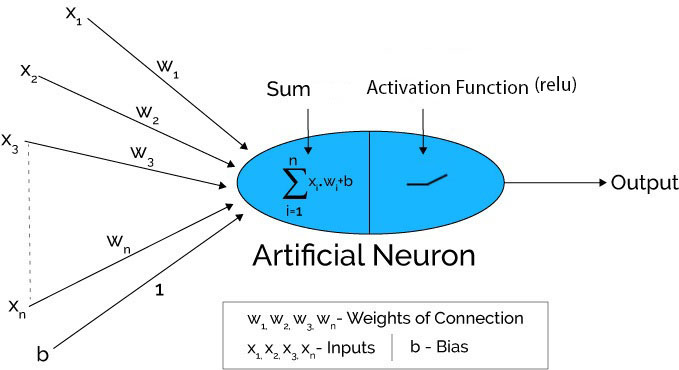
\includegraphics[width=16.5cm]{./images/image2.jpg}
\label{neuroneSeul}
\caption{Fonctionnement d'un neurone seul}
\end{figure}

Notre apprentissage se fera en modifiant les poids de ses différentes
connexions (et le biais) de façon à obtenir une sortie proche de celle voulu.\newline

\hypertarget{Ruxe9seau-de-neurones-classique}{%
\subsection{Réseau de neurones classique}
\label{Ruxe9seau-de-neurones-classique}}

Les neurones présentés précédemment prennent tout leur intérêt lorsqu'ils sont utilisés en groupes, dans des \textbf{réseaux de neurones}.

Le premier de ces réseaux, encore utilisé de nos jours, est appelé \textbf{perceptron}.
Le principe du perceptron n'est pas nouveau et date des années 1960.

Dans ces réseaux, les neurones sont organisés en \textbf{couches}.
La première couche correspond à celle qui permettra d'introduire des informations dans le réseau (comme la rétine par exemple). Elle est nommée \textbf{couche d'entrée}
La dernière couche permettra de lire les décisions du réseau. Elle est appelée \textbf{couche de sortie}. Dans les applications classiques, à chaque neurone de la couche de sortie correspond une décision possible et le neurone qui est le plus activé sur la couche de sortie l'emporte.
Entre ces couches, on trouve souvent un nombre variable de couches intermédiaires appelées \textbf{couches cachées}.

Entre deux couches, on établit le plus souvent un schéma de connexion que nous pouvons qualifier de \textit{full connected}, c'est à dire que chaque neurone d'une couche est connecté avec chaque neurone de la couche suivante.Nous allons encore une fois, pour le bien de ce rapport, ne pas épiloguer sur les autres types de connexions existantes.\newline

Nous allons, pour cette partie encore, utiliser une figure (\ref{reseauClassique}) pour illustrer nos propos:

\begin{figure}[h]
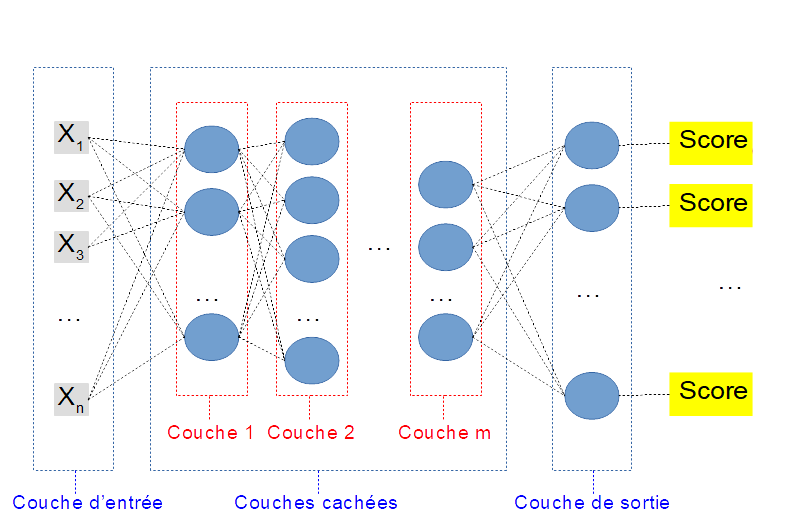
\includegraphics[width=16.5cm]{./images/multicouche.png}
\caption{réseau de neurones classique en couches}
\label{reseauClassique}
\end{figure}


\hypertarget{Ruxe9seau-de-neurones-convolutif}{%
\subsection{Réseau de neurones convolutifs}
\label{Ruxe9seau-de-neurones-convolutif}}

le réseau de neurones convolutifs est un type de réseau de neurones
inspiré par le cortex cérébral des animaux.
Il possède de larges applications dans la reconnaissance d'image, de vidéo et de son.

Ce réseau se présente comme un réseau classique , une couche d'entrée,
une couche de sortie et des couches cachées.
Ces couches cachées possèdent des couches \textbf{convolutives}
pour lesquelles chaque neurone va appliquer un filtre convolutif
sur une partie de l'image en entrée afin d'analyser toute l'image
(voir figure \ref{fig:explication_convolution}).

\begin{figure}[h!]
\begin{center}
\centering
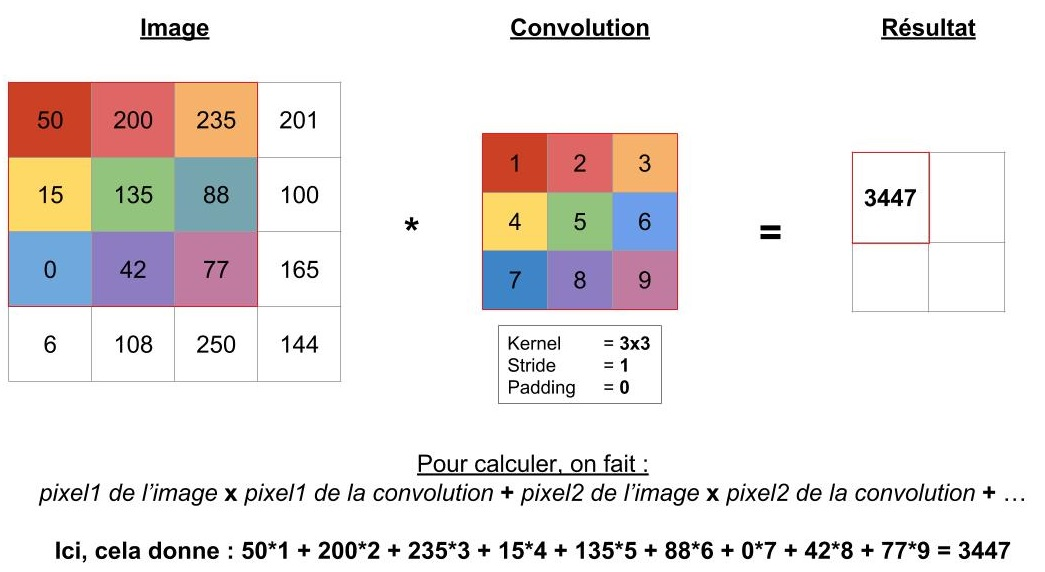
\includegraphics[width=15cm]{./images/explication_convolution.jpg}
\caption[Schéma de la convolution.]{L'image d'entrée est découpée en \textit{patchs}
sur lesquels est appliqué un filtre de convolution.
La sortie de ce fitre appliqué à chacun des patchs donne la couche de sortie
de la couche convolutive (appelée carte ou map).
La convolution est paramètrée par : le \textit{kernel} (la forme du patch),
le \textit{stride} (le déplacement du filtre) et le \textit{padding}
 (la façon dont les bords de l'image vont être traités).\label{fig:explication_convolution}}
\end{center}
\end{figure}

Ces neurones ont souvent une fonction d'activation \textit{relu}
qui borne l'activation du neurone à 0. Ce sont donc des neurones
dont l'activation ne peut être que positive.

Les réseaux convolutifs possèdent aussi des couches de \textbf{pooling}.
Le \textbf{pooling} est une opération simple qui consiste à remplacer une zone de pixels
(généralement 2×2 ou 3×3) par une valeur unique (généralement le max ou la moyenne).
De cette manière, l’image diminue en taille et se retrouve simplifiée (lissée).

L'intérêt majeur des réseaux convolutifs est qu'ils permettent de réaliser une invariance
de translation : un motif appris sur une zone de l'image sera reconnue
quelque soit sa position dans l'image.

\hypertarget{Tensorflow}{%
\subection{TensorFlow}
\label{Tensorflow}}

\begin{center}
\label{fig:Tensorflow_logo}
\centering

\includegraphics[width=5cm]{./images/Tensorflow_logo.png}
\begin{figure}[h!]
\caption{Logo de Tensorflow}
\end{figure}
\end{center}


TensorFlow est un framework open source,
multiplateforme d'apprentissage automatique développée par Google Brain,
en Python et en C++.
Sa premiere version est publiée par Google le 9 novembre 2015.
L'intérêt de ce framework est de limiter les coûts de développement des solutions à base
de réseaux de neurones, en réunissant des fonctionnalités permettant,
en quelques lignes de code de construire des réseaux complexes.
Tensorflow permet donc de simplifier beaucoup de choses dans
le domaine de l'apprentissage automatique.
Son autre intérêt est de fournir des interfaces pour pouvoir exécuter les calculs sur
des accélérateurs graphiques et surtout de les prendre en charge
de façon complétement transparente pour les utilisateurs.
Les gains de vitesse peuvent atteindre ainsi un facteur 10 quand le même modèle est exécuté
sur une carte graphique.

\hypertarget{plan}{%
\Chapter{Présentation du plan du rapport}\label{Présentation du plan du rapport}}
